\documentclass[a4paper,12pt]{article}
\usepackage[top=1in, bottom=1.5in, left=1in, right=1in]{geometry}
\usepackage[utf8]{inputenc}
\usepackage{natbib}
\usepackage{graphicx}
\usepackage{amsmath, amssymb, amsfonts}
\usepackage{wrapfig}
\usepackage{xcolor}
\usepackage{caption}
\usepackage{enumitem}
\usepackage{hyperref}
\hypersetup{
    colorlinks = true,
    linkcolor = black,
    urlcolor  = blue,
    citecolor = gray
}
\graphicspath{{../images/}}
\setlength{\parindent}{0cm} % Remove automatic indentation
\setlength{\parskip}{1em}
\captionsetup[figure]{font=small,skip=1pt}

\begin{document}

    \begin{titlepage}
        \begin{center}
            \vspace*{2cm}

            \huge
            \textbf{Principal Component Analysis}

            \vspace{0.5cm}
            \LARGE
            Pulsar Stars

            \vspace{2cm}

            \textbf{Marina Tihova}\\
            mtt862@student.bham.ac.uk

            \vspace{1.5cm}

            
\includegraphics[height=.3\textwidth, width=0.3\textwidth]{logo}

            \large
            School of Computer Science\\
            Computer Science BSc\\
            University of Birmingham\\
            March, 2020

        \end{center}
    \end{titlepage}

    \newpage

    \tableofcontents
    \newpage


    \section{What is PCA?}
    In the real world, datasets may contain hundreds of attributes and naturally, some attributes will be more important than others. PCA aims to help with simplifying high-dimensional data by reducing the number of dimensions while preserving the essence of the data. \par
    In order to reduce the dimensionality of the feature space PCA introduces new variables (principal components) that are orthogonal to each other. A principal component is a linear combination of the original predictor variables which captures the maximum variance in the data set. A downside of the resulting principal components being a complex mixture of the original features is that interpreting them can prove difficult.\par
    Usually PCA is used before applying machine learning algorithms. When the input dimension is too high, PCA can speed up the process. It can also combat overfitting by filtering the irrelevant attributes which decrease the performance of some algorithms. Another common use for PCA is data visualisation since understanding two- or three-dimensional data is not as challenging as higher dimensional data.\par


    \newpage

    \section{Dataset}
    \subsection{Introduction}
    I decided to use the HTRU2 dataset with the goal of predicting a pulsar star. HTRU2 is a data set which describes a sample of pulsar candidates collected during the High Time Resolution Universe Survey.\cite{highTimeResolution}  \par
    The dataset contains a “target class” attribute explaining which samples are pulsar stars and which are not. In practice, almost all detections are caused by radio frequency interference (RFI) and noise, making legitimate signals hard to find. HTRU2 contains 16,259 spurious examples caused by RFI/noise, and 1,639 real pulsar examples. I’ll be plotting the “target” attribute against the others in order to find pulsar stars.\cite{htru2}

    \subsection{What are pulsar stars?}
    Pulsars are a rare type of Neutron star meaning they are exceptionally small and dense. Their interesting properties make them a significant point of interest for a plethora of scientists.

    \begin{figure}[ht]
        \centering
        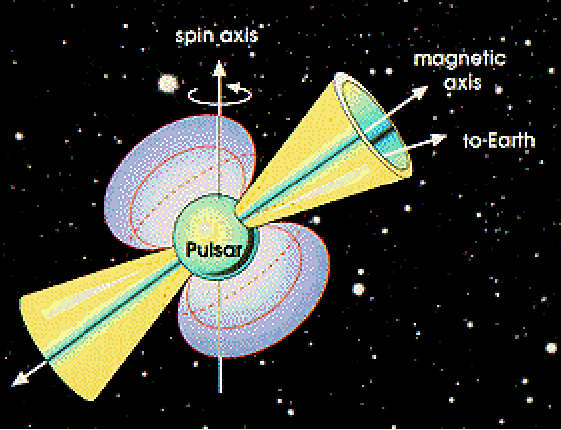
\includegraphics[scale=.85]{pulsar}
        \caption{Pulsar star \textit{(Image credit: NASA)}}
        \label{fig:pulsar}
    \end{figure}

    \newpage

    \subsection{Properties}
    Pulsars radiate two steady, narrow beams of light in opposite directions. Although the light from the beam is steady, pulsars appear to flicker because they also spin. It’s often compared to when a lighthouse appears to blink when seen by a sailor on the ocean: as the pulsar rotates, the beam of light may sweep across the Earth, then swing out of view, then swing back around again.\cite{pulsarSpace}\par

    \begin{figure}[ht]
        \centering
        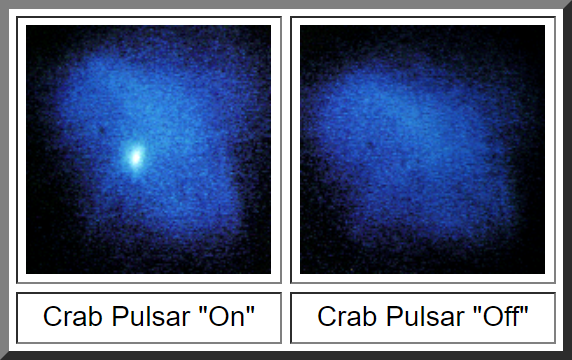
\includegraphics[width=.5\textwidth]{pulsar-blink}
        \caption{\textit{(Image credit: Einstein X-ray observatory)}}
        \label{fig:blinkingpulsar}
    \end{figure}

    Pulsars are highly magnetic. Their magnetic fields range from 100 million times to 1 quadrillion times stronger than Earth's.\cite{pulsarWiki}

    \subsection{Applications}
    Pulsars are fantastic cosmic tools for scientists to study a wide range of phenomena.\par
    Many pulsars blink with extreme precision. Pulsars can be used as precise clocks since they are considered the most accurate natural clocks in the universe.\par
    Because pulsars are moving through space while also blinking a regular number of times per second, scientists can use many pulsars to calculate cosmic distances. Thanks to the exquisite timing of the pulses, scientists have made some of the most accurate distance measurements of cosmic objects.\par
    The physics of neutron stars can be researched by analysing the light emitted by a pulsar. Because of their density, matter around them behaves in new unexpected ways.\par
    Pulsars have also been used to test aspects of Albert Einstein's theory of general relativity, such as the universal force of gravity.\cite{pulsarSpace}
    \newpage

    \subsection{Attributes}
    \subsubsection{Integrated pulse profile (folded profile)}
    Pulsars produce periodic pulsation signals which are often too weak to detect. Integrated pulsar signals (with respect to its rotational period) increase the signal quality and form integrated pulse profile. Pulsars are distinguished by their \textit{integrated pulse profiles} – all pulsars have their unique profile shape, similar to human’s fingerprints. \cite{integratedProfile} \\
    The HTRU2 dataset includes:
    \begin{enumerate}
        \item Mean of the integrated profile
        \item Standard deviation of the integrated profile
        \item Excess kurtosis of the integrated profile
        \item Skewness of the integrated profile
    \end{enumerate}

    \subsubsection{DM-SNR curve}
    When observing a pulsar over a finite bandwidth, a broadening of an otherwise sharp pulse can be seen. This is the \textit{dispersion measure (DM)}. DM is a constant defined by the column density of free electrons along the line of sight. The DM-SNR curve describes the dispersion measure given the signal to noise ratio of the integrated profile.\cite{dmstr} \\
    The HTRU2 dataset includes:
    \begin{enumerate}[resume]
        \item Mean of the DM-SNR curve
        \item Standard deviation of the DM-SNR curve
        \item Excess kurtosis of the DM-SNR curve
        \item Skewness of the DM-SNR curve
    \end{enumerate}

    \subsubsection{Target class}
    The HTRU2 dataset includes:
    \begin{enumerate}[resume]
        \item Target class
        \begin{itemize}
            \item Label 1: indicating the sample is a real pulsar
            \item Label 0: indicating the sample is spurious
        \end{itemize}
    \end{enumerate}
    \newpage

    \section{Expectations}
    I expect to discover that not all dataset features are as important to predicting a pulsar star. By applying PCA to this dataset, hopefully, the results will show that in practice the star data is less dimensional and more reliant on certain features than others.\par
    When plotting the data over the first few principal components I expect to see clear separation between the spurious and pulsar star samples. This implies that if I plugged a new sample in and plotted it on the same projection, I’d be able to see whether it has features making it more prone to be either a real pulsar or just a frequency noise.\par

    \section{Software}
    I decided to use Python for conducting PCA. After researching various approaches for PCA, such as \textit{Python}, \textit{MATLAB}, or the language \textit{R}, and writing sample code in them, I found Python to be the most convenient and versatile approach for me. Python contains tools for handling huge matrices, performing large computations and is often used for machine learning purposes.\par
    For this project I used \textit{IPython} alongside \textit{Jupyter Notebook} for applying PCA, plotting projections, and documenting the process using markdown language. The libraries I relied on were:
    \begin{itemize}
        \item \textbf{pandas} for data manipulation. Pandas supplied me with an appealing way to visualise two dimensional matrices and to modify a dataset in terms of a table with an index and columns.
        \item \textbf{numpy} for the large collection of high-level mathematical functions they provide. Pandas works closely with numpy for handing multi-dimensional arrays.
        \item \textbf{scikit-learn} because it features various classification, regression and clustering algorithms including PCA.
        \item \textbf{matplotlib} to plot the results.
    \end{itemize}
    Furthermore, Python was the best choice for me since I've extensively used pandas and numpy in my experience prior university. All the code I wrote for this project can be found in my \href{https://github.com/MarchiT/pulsar-pca}{GitHub} repository.
    \newpage

    \section{Pre-processing of the data}
    Before my final dataset choice, I tried a few more datasets which had a lot of categorical data columns. After converting to numerical values, I discovered that said datasets were complex and too dependent of all features thus making them not suitable for finding interesting results via PCA. Excluding the target class, the pulsar dataset has only numerical values and conversion was not needed in this case.\par
    Before starting PCA, I removed the target class column from the dataset table so it wouldn't throw off the data.\par
    After removing the class, I normalised the data.
    \[X_{scaled} = \frac{X - m}{\sqrt{Variance}}\]
    The values before and after scaling for the first 5 samples are as follows:

    \begin{figure}[ht]
        \centering
        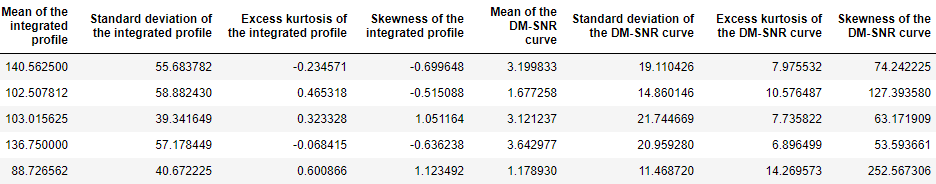
\includegraphics[width=\textwidth]{df-before-scaling}
        \caption{Data before scaling}
    \end{figure}

    \begin{figure}[ht]
        \centering
        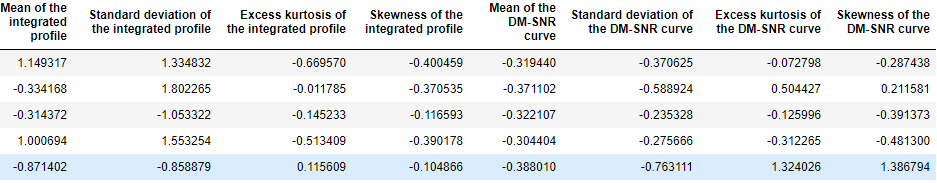
\includegraphics[width=\textwidth]{df-after-scaling}
        \caption{Data after scaling}
    \end{figure}

    The next 6 figures display information for the mean, variance and covariance before and after normalisation respectively.

    \newpage

    \begin{figure}[ht!]
        \begin{math}
            \begin{array}{lcr}
                \mbox{ Mean of the integrated profile} & 111.07996834492681 \\
                \mbox{ Standard deviation of the integrated profile} & 46.549531561534295 \\
                \mbox{ Excess kurtosis of the integrated profile} & 0.4778572581019128 \\
                \mbox{ Skewness of the integrated profile} & 1.7702789980713511 \\
                \mbox{ Mean of the DM-SNR curve} & 12.614399658311525 \\
                \mbox{ Standard deviation of the DM-SNR curve} & 26.326514703918694 \\
                \mbox{ Excess kurtosis of the DM-SNR curve} & 8.303556116638275 \\
                \mbox{ Skewness of the DM-SNR curve} & 104.85770870366196 \\
            \end{array}
        \end{math}
        \caption{Mean before normalisation}
    \end{figure}

    \begin{figure}[ht!]
        \begin{math}
            \begin{array}{lcr}
                \mbox{ Mean of the integrated profile} & -0 \\
                \mbox{ Standard deviation of the integrated profile} & -0 \\
                \mbox{ Excess kurtosis of the integrated profile} & 0 \\
                \mbox{ Skewness of the integrated profile} & 0 \\
                \mbox{ Mean of the DM-SNR curve} & -0 \\
                \mbox{ Standard deviation of the DM-SNR curve} & 0 \\
                \mbox{ Excess kurtosis of the DM-SNR curve} & 0 \\
                \mbox{ Skewness of the DM-SNR curve} & 0 \\
            \end{array}
        \end{math}
        \caption{Mean after normalisation (to 10 decimal places)}
    \end{figure}

    \begin{figure}[ht!]
        \begin{math}
            \begin{array}{lcr}
                \mbox{ Mean of the integrated profile} & 658.0363246090876 \\
                \mbox{ Standard deviation of the integrated profile} & 46.82662485126457 \\
                \mbox{ Excess kurtosis of the integrated profile} & 1.1321172606433363 \\
                \mbox{ Skewness of the integrated profile} & 38.04102827819613 \\
                \mbox{ Mean of the DM-SNR curve} & 868.603132969526 \\
                \mbox{ Standard deviation of the DM-SNR curve} & 379.08200556314085 \\
                \mbox{ Excess kurtosis of the DM-SNR curve} & 20.30372936498847 \\
                \mbox{ Skewness of the DM-SNR curve} & 11344.713243182858 \\
            \end{array}
        \end{math}
        \caption{Variance before normalisation}
    \end{figure}

    \begin{figure}[ht!]
        \begin{math}
            \begin{array}{lcr}
                \mbox{ Mean of the integrated profile} & 1 \\
                \mbox{ Standard deviation of the integrated profile} & 1 \\
                \mbox{ Excess kurtosis of the integrated profile} & 1 \\
                \mbox{ Skewness of the integrated profile} & 1 \\
                \mbox{ Mean of the DM-SNR curve} & 1 \\
                \mbox{ Standard deviation of the DM-SNR curve} & 1 \\
                \mbox{ Excess kurtosis of the DM-SNR curve} & 1 \\
                \mbox{ Skewness of the DM-SNR curve} & 1 \\
            \end{array}
        \end{math}
        \caption{Variance after normalisation}
    \end{figure}

    \newpage

    \setcounter{MaxMatrixCols}{20}
    \begin{figure}[ht!]
        \centering
        \begin{math}
            \begin{bmatrix}
                658.07&96.05&-23.85&-116.89&-225.94&-153.35&27.09&393.56\\
                96.05&46.83&-3.8&-22.78&1.39&-6.35&0.91&20.18\\
                -23.85&-3.8&1.13&6.21&12.99&8.97&-1.64&-24.31\\
                -116.89&-22.78&6.21&38.04&74.91&49.86&-9.14&-134.54\\
                -225.94&1.39&12.99&74.91&868.65&457.11&-81.81&-1112.15\\
                -153.35&-6.35&8.97&49.86&457.11&379.1&-71.05&-1194.15\\
                27.09&0.91&-1.64&-9.14&-81.81&-71.05&20.3&443.36\\
                393.56&20.18&-24.31&-134.54&-1112.15&-1194.15&443.36&11345.35
            \end{bmatrix}
        \end{math}
        \caption{Covariance Matrix before normalisation (to 2 decimal places)}
    \end{figure}

    \setcounter{MaxMatrixCols}{20}
    \begin{figure}[ht!]
        \centering
        \begin{math}
            \begin{bmatrix}
                1.0&0.55&-0.87&-0.74&-0.3&-0.31&0.23&0.14\\
                0.55&1.0&-0.52&-0.54&0.01&-0.05&0.03&0.03\\
                -0.87&-0.52&1.0&0.95&0.41&0.43&-0.34&-0.21\\
                -0.74&-0.54&0.95&1.0&0.41&0.42&-0.33&-0.2\\
                -0.3&0.01&0.41&0.41&1.0&0.8&-0.62&-0.35\\
                -0.31&-0.05&0.43&0.42&0.8&1.0&-0.81&-0.58\\
                0.23&0.03&-0.34&-0.33&-0.62&-0.81&1.0&0.92\\
                0.14&0.03&-0.21&-0.2&-0.35&-0.58&0.92&1.0
            \end{bmatrix}
        \end{math}
        \caption{Covariance Matrix after normalisation (to 2 decimal places)}
    \end{figure}

    \newpage

    \section{Insights}

    \begin{figure}[ht]
        \centering
        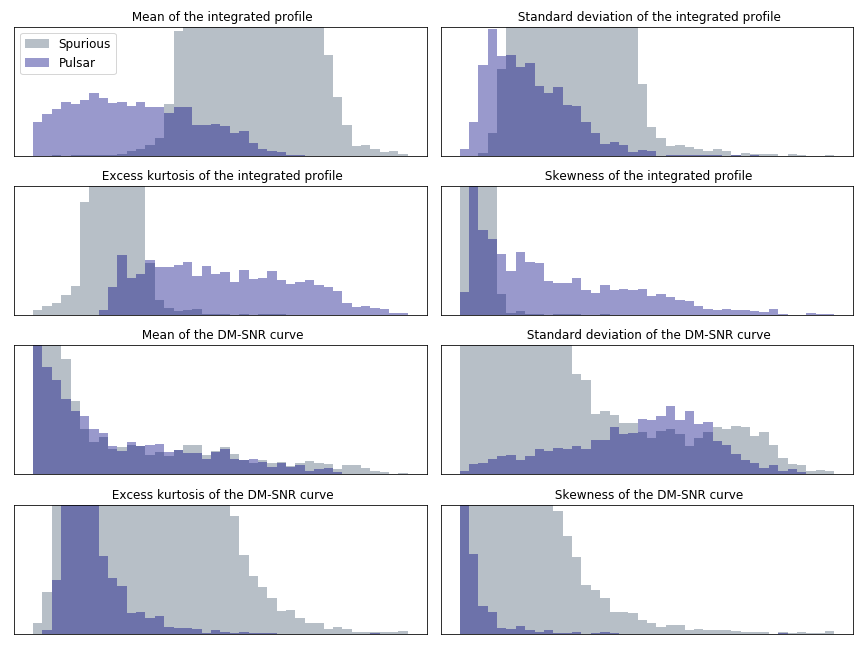
\includegraphics[width=\textwidth]{insights}
        \caption{Target histograms}
        \label{fig:insights}
    \end{figure}

    The results of plotting projections of the data onto pairs of its existing dimensions can be seen on Figure ~\ref{fig:insights}. Since the number of spurious examples in the dataset is significantly larger than the true stars, I had to limit the y axis so the overlap can be shown more clearly in the plots. \par
    The projections reveal that the \textbf{DM-SNR curve} values don’t hold much essential information due to the targets mostly overlapping in said plots. Both targets describe similar values for their DM-SNR curves therefore using only the DM-SNR curve data won’t be enough to distinguish noise from a real pulsar star using PCA. \par
    Observing the \textbf{integrated profile} plots shows us that there’s a difference in the two targets. The \textit{skewness} and \textit{excess kurtosis} of the integrated profile for the pulsar stars seem to be generally higher than the spurious stars. The \textit{mean} and the \textit{standard deviation} on the other hand usually take on lower values for the pulsars. The integrated profile features will prove more crucial and will contribute more when applying PCA. This shows us that the data is potentially less dimensional than it appears to be.

    \newpage

    \section{Calculations}

    \subsection{Covariance Matrix}

    \setcounter{MaxMatrixCols}{20}
    \begin{figure}[h]
        \centering
        \begin{math}
            \begin{bmatrix}
                4.13428&0.0&-0.0&0.0&-0.0&-0.0&0.0&-0.0\\
                0.0&2.14472&0.0&0.0&-0.0&0.0&-0.0&-0.0\\
                -0.0&0.0&0.80939&-0.0&0.0&0.0&-0.0&-0.0\\
                0.0&0.0&-0.0&0.45745&0.0&0.0&0.0&0.0\\
                -0.0&-0.0&0.0&0.0&0.25824&0.0&0.0&0.0\\
                -0.0&0.0&0.0&0.0&0.0&0.15989&-0.0&0.0\\
                0.0&-0.0&-0.0&0.0&0.0&-0.0&0.02044&0.0\\
                -0.0&-0.0&-0.0&0.0&0.0&0.0&0.0&0.01603
            \end{bmatrix}
        \end{math}
        \caption{Covariance Matrix after PCA (to 5 decimal places)}
    \end{figure}

    \subsection{Eigenvalues and Eigenvectors}

    \setcounter{MaxMatrixCols}{20}
    \begin{figure}[h]
        \centering
        \begin{math}
            \begin{array}{c}
                4.134277694661789\cr2.144724928035271\cr0.8093941863429204\cr0.4574503833736197\cr0.25824134528449544\cr0.1598882366882819\cr0.020443080572961073\cr0.016027147331548922
            \end{array}
        \end{math}
        \caption{Eigenvalues}
    \end{figure}

    \setcounter{MaxMatrixCols}{20}
    \begin{figure}[h]
        \centering
        \begin{math}
            \begin{bmatrix}
                0.36&0.36&0.01&0.29&0.74&0.02&0.31&-0.03\\
                0.21&0.43&-0.44&-0.76&0.02&0.05&-0.06&-0.0\\
                -0.42&-0.32&-0.09&-0.3&0.15&0.05&0.77&-0.06\\
                -0.4&-0.31&-0.08&-0.18&0.64&-0.02&-0.54&0.03\\
                -0.35&0.25&-0.57&0.33&-0.07&-0.61&0.03&-0.09\\
                -0.39&0.32&-0.23&0.26&-0.07&0.75&-0.06&-0.24\\
                0.37&-0.41&-0.27&0.04&0.0&0.02&-0.05&-0.78\\
                0.29&-0.4&-0.58&0.2&-0.02&0.25&0.03&0.56
            \end{bmatrix}
        \end{math}
        \caption{Eigenvectors (to 2 decimal places)}
    \end{figure}

    \begin{figure}[ht!]
        \centering
        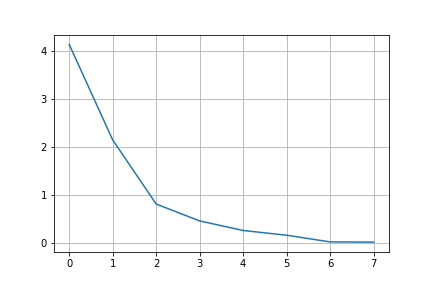
\includegraphics[clip, trim = 0 0 0 1cm, width=.75\textwidth]{eigen}
        \caption{Eigenvalues plotted}
        \label{fig:eigenvalues-plot}
    \end{figure}

    \newpage

    The eigenvalues plot on Figure ~\ref{fig:eigenvalues-plot} clearly shows that the first 3 eigenvalues explain most of the data. After calculating the explained variance ratio, we can see that the 1\textsuperscript{st}, 2\textsuperscript{nd}, and 3\textsuperscript{rd} principal components reveal 52\%, 79\%, 89\% of the data respectively (see Figure ~\ref{fig:eigenvalues-plot-percent}). Thus, by using the first 3 components for the final projection, the plot would have access to nearly 90\% of the information.

    \begin{figure}[ht!]
        \centering
        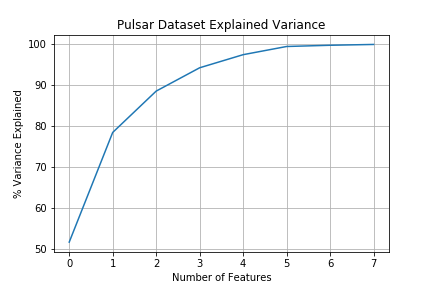
\includegraphics[width=.75\textwidth]{eigen-percent}
        \caption{\% Explained variance}
        \label{fig:eigenvalues-plot-percent}
    \end{figure}

    \newpage

    \subsection{Final Projections}

    \begin{figure}[ht!]
        \centering
        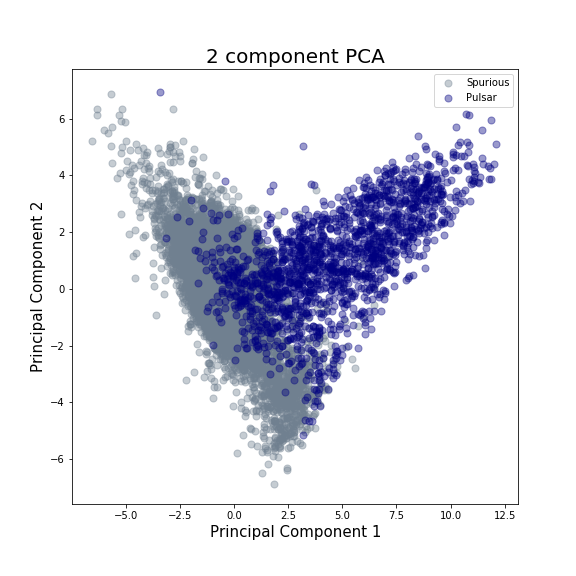
\includegraphics[clip, trim = 0 1cm 0 1.7cm, height=.61\textwidth]{2component-projection}
        \caption{2-component projection}
    \end{figure}

    \begin{figure}[ht!]
        \centering
        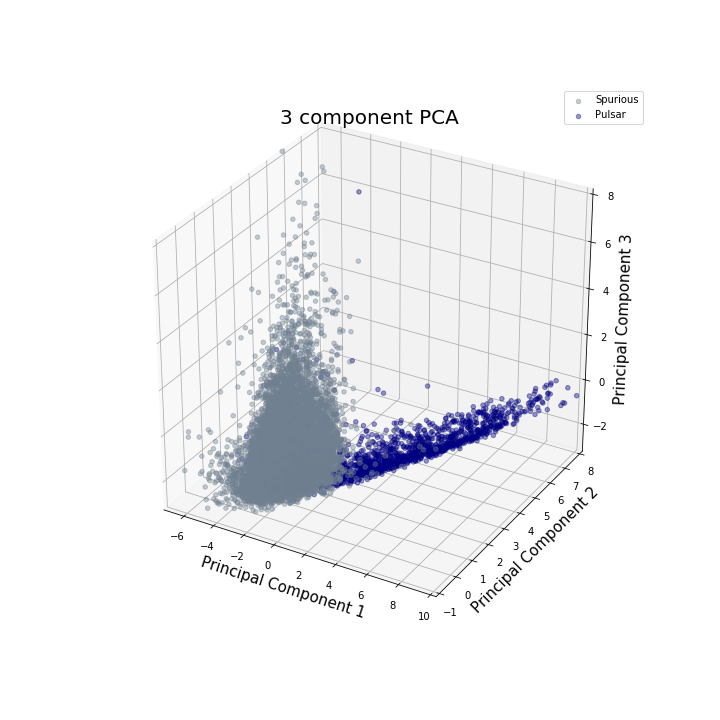
\includegraphics[clip, trim = 0 3.5cm 0 3.2cm, height=.666\textwidth]{3component-projection}
        \caption{3-component projection}
    \end{figure}

    \newpage

    \subsection{Explaining the projections}

    \section{Conclusion}

    \newpage

    \bibliographystyle{unsrt}
    \bibliography{references}
\end{document}
